% Generated by code/needham.py -- do not edit by hand.
\definecolor{qocA}{rgb}{0.00,0.45,0.70}
\definecolor{qocB}{rgb}{0.90,0.60,0.00}
\definecolor{qocC}{rgb}{0.00,0.62,0.45}
\definecolor{qocD}{rgb}{0.80,0.40,0.00}
\definecolor{qocE}{rgb}{0.80,0.60,0.70}
\definecolor{qocF}{rgb}{0.35,0.70,0.90}
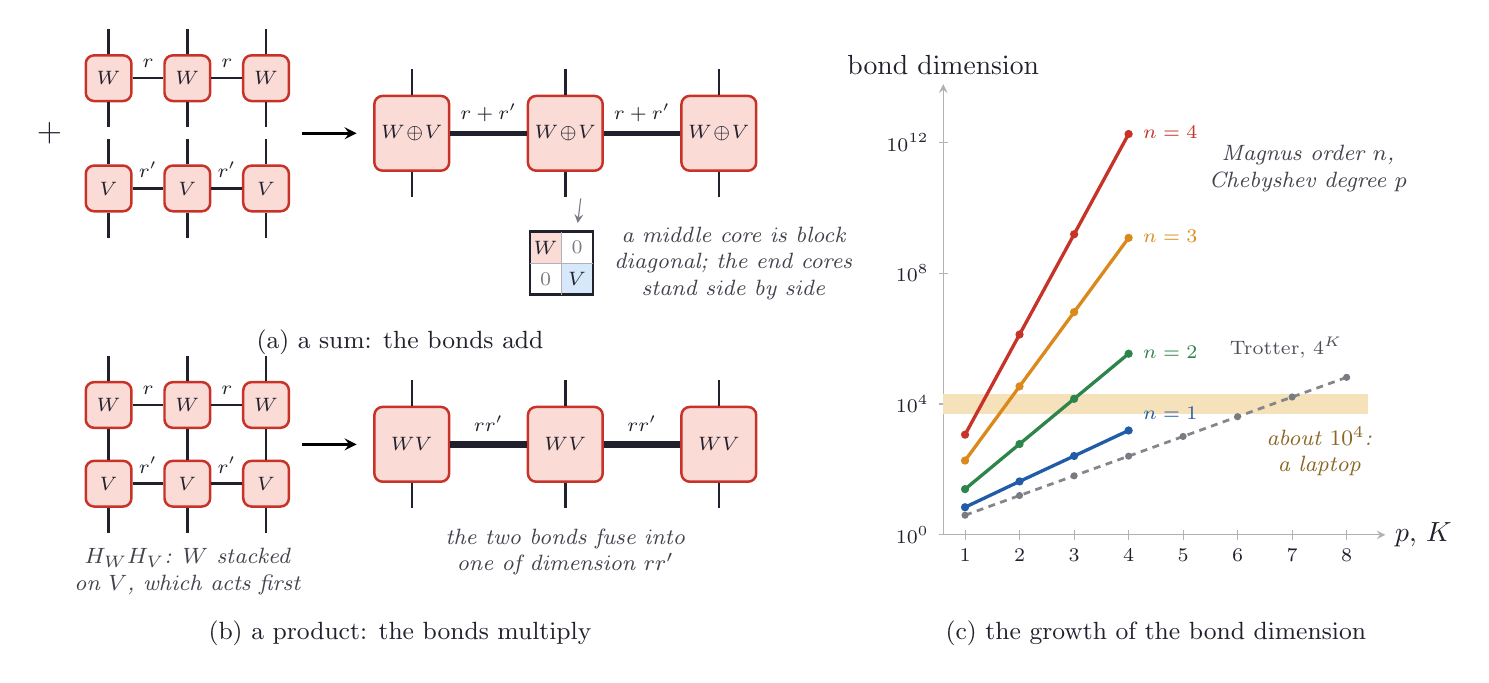
\begin{tikzpicture}[ink/.style={line width=0.9pt, ndInk}, faint/.style={line width=0.4pt, ndInk!35}, dashedink/.style={line width=0.5pt, ndInk!55, dash pattern=on 2.5pt off 2pt}, vec/.style={->, >=stealth, line width=1.2pt}, note/.style={font=\footnotesize\itshape, text=ndInk!85, align=center}, pointer/.style={->, >=stealth, line width=0.4pt, ndInk!60, shorten >=2pt, shorten <=1pt}, dot/.style={circle, fill=ndInk, inner sep=0pt, minimum size=3.4pt}, wash/.style={fill=ndSky, fill opacity=0.55}, every node/.style={text=ndInk}]
\definecolor{ndInk}{rgb}{0.13,0.13,0.18}
\definecolor{ndPaper}{rgb}{0.99,0.96,0.88}
\definecolor{ndSky}{rgb}{0.84,0.91,0.98}
\definecolor{ndRose}{rgb}{0.98,0.86,0.84}
\definecolor{ndBlue}{rgb}{0.13,0.36,0.66}
\definecolor{ndRed}{rgb}{0.78,0.20,0.16}
\definecolor{ndGold}{rgb}{0.88,0.62,0.10}
\definecolor{ndGreen}{rgb}{0.18,0.52,0.30}
\node[rectangle, rounded corners=3pt, minimum size=0.58cm, fill=ndRose, draw=ndRed, line width=0.9pt, font=\scriptsize, inner sep=1pt] (a0) at (0.600,6.900) {$W$};
\draw[ink] (a0.north) -- ++(0,0.32);
\draw[ink] (a0.south) -- ++(0,-0.32);
\node[rectangle, rounded corners=3pt, minimum size=0.58cm, fill=ndRose, draw=ndRed, line width=0.9pt, font=\scriptsize, inner sep=1pt] (a1) at (1.600,6.900) {$W$};
\draw[ink] (a1.north) -- ++(0,0.32);
\draw[ink] (a1.south) -- ++(0,-0.32);
\node[rectangle, rounded corners=3pt, minimum size=0.58cm, fill=ndRose, draw=ndRed, line width=0.9pt, font=\scriptsize, inner sep=1pt] (a2) at (2.600,6.900) {$W$};
\draw[ink] (a2.north) -- ++(0,0.32);
\draw[ink] (a2.south) -- ++(0,-0.32);
\draw[ndInk, line width=0.9pt] (a0.east) -- node[above, font=\scriptsize] {$r$} (a1.west);
\draw[ndInk, line width=0.9pt] (a1.east) -- node[above, font=\scriptsize] {$r$} (a2.west);
\node[rectangle, rounded corners=3pt, minimum size=0.58cm, fill=ndRose, draw=ndRed, line width=0.9pt, font=\scriptsize, inner sep=1pt] (v0) at (0.600,5.500) {$V$};
\draw[ink] (v0.north) -- ++(0,0.32);
\draw[ink] (v0.south) -- ++(0,-0.32);
\node[rectangle, rounded corners=3pt, minimum size=0.58cm, fill=ndRose, draw=ndRed, line width=0.9pt, font=\scriptsize, inner sep=1pt] (v1) at (1.600,5.500) {$V$};
\draw[ink] (v1.north) -- ++(0,0.32);
\draw[ink] (v1.south) -- ++(0,-0.32);
\node[rectangle, rounded corners=3pt, minimum size=0.58cm, fill=ndRose, draw=ndRed, line width=0.9pt, font=\scriptsize, inner sep=1pt] (v2) at (2.600,5.500) {$V$};
\draw[ink] (v2.north) -- ++(0,0.32);
\draw[ink] (v2.south) -- ++(0,-0.32);
\draw[ndInk, line width=0.9pt] (v0.east) -- node[above, font=\scriptsize] {$r'$} (v1.west);
\draw[ndInk, line width=0.9pt] (v1.east) -- node[above, font=\scriptsize] {$r'$} (v2.west);
\node[font=\large] at (-0.15,6.2) {$+$};
\draw[->, >=stealth, line width=0.9pt] (3.05,6.2) -- (3.75,6.2);
\node[rectangle, rounded corners=3pt, minimum size=0.95cm, fill=ndRose, draw=ndRed, line width=0.9pt, font=\scriptsize, inner sep=1pt] (s0) at (4.450,6.200) {$W\!\oplus\!V$};
\draw[ink] (s0.north) -- ++(0,0.32);
\draw[ink] (s0.south) -- ++(0,-0.32);
\node[rectangle, rounded corners=3pt, minimum size=0.95cm, fill=ndRose, draw=ndRed, line width=0.9pt, font=\scriptsize, inner sep=1pt] (s1) at (6.400,6.200) {$W\!\oplus\!V$};
\draw[ink] (s1.north) -- ++(0,0.32);
\draw[ink] (s1.south) -- ++(0,-0.32);
\node[rectangle, rounded corners=3pt, minimum size=0.95cm, fill=ndRose, draw=ndRed, line width=0.9pt, font=\scriptsize, inner sep=1pt] (s2) at (8.350,6.200) {$W\!\oplus\!V$};
\draw[ink] (s2.north) -- ++(0,0.32);
\draw[ink] (s2.south) -- ++(0,-0.32);
\draw[ndInk, line width=1.6pt] (s0.east) -- node[above, font=\scriptsize] {$r+r'$} (s1.west);
\draw[ndInk, line width=1.6pt] (s1.east) -- node[above, font=\scriptsize] {$r+r'$} (s2.west);
\fill[ndRose] (5.95,4.55) rectangle (6.35,4.95);
\fill[ndSky] (6.35,4.15) rectangle (6.75,4.55);
\draw[ink] (5.95,4.15) rectangle (6.75,4.95);
\draw[faint] (6.35,4.15) -- (6.35,4.95) (5.95,4.55) -- (6.75,4.55);
\node[font=\scriptsize] at (6.15,4.75) {$W$};
\node[font=\scriptsize] at (6.55,4.35) {$V$};
\node[font=\scriptsize, text=ndInk!60] at (6.55,4.75) {$0$};
\node[font=\scriptsize, text=ndInk!60] at (6.15,4.35) {$0$};
\draw[pointer] (s1.south) ++(0.2,-0.3) -- (6.55,4.99);
\node[note, anchor=west] at (6.90,4.55) {a middle core is block\\ diagonal; the end cores\\ stand side by side};
\node[font=\small] at (4.3,3.55) {(a) a sum: the bonds add};
\node[rectangle, rounded corners=3pt, minimum size=0.58cm, fill=ndRose, draw=ndRed, line width=0.9pt, font=\scriptsize, inner sep=1pt] (p0) at (0.600,2.750) {$W$};
\draw[ink] (p0.north) -- ++(0,0.32);
\node[rectangle, rounded corners=3pt, minimum size=0.58cm, fill=ndRose, draw=ndRed, line width=0.9pt, font=\scriptsize, inner sep=1pt] (p1) at (1.600,2.750) {$W$};
\draw[ink] (p1.north) -- ++(0,0.32);
\node[rectangle, rounded corners=3pt, minimum size=0.58cm, fill=ndRose, draw=ndRed, line width=0.9pt, font=\scriptsize, inner sep=1pt] (p2) at (2.600,2.750) {$W$};
\draw[ink] (p2.north) -- ++(0,0.32);
\draw[ndInk, line width=0.9pt] (p0.east) -- node[above, font=\scriptsize] {$r$} (p1.west);
\draw[ndInk, line width=0.9pt] (p1.east) -- node[above, font=\scriptsize] {$r$} (p2.west);
\node[rectangle, rounded corners=3pt, minimum size=0.58cm, fill=ndRose, draw=ndRed, line width=0.9pt, font=\scriptsize, inner sep=1pt] (q0) at (0.600,1.750) {$V$};
\draw[ink] (q0.south) -- ++(0,-0.32);
\node[rectangle, rounded corners=3pt, minimum size=0.58cm, fill=ndRose, draw=ndRed, line width=0.9pt, font=\scriptsize, inner sep=1pt] (q1) at (1.600,1.750) {$V$};
\draw[ink] (q1.south) -- ++(0,-0.32);
\node[rectangle, rounded corners=3pt, minimum size=0.58cm, fill=ndRose, draw=ndRed, line width=0.9pt, font=\scriptsize, inner sep=1pt] (q2) at (2.600,1.750) {$V$};
\draw[ink] (q2.south) -- ++(0,-0.32);
\draw[ndInk, line width=0.9pt] (q0.east) -- node[above, font=\scriptsize] {$r'$} (q1.west);
\draw[ndInk, line width=0.9pt] (q1.east) -- node[above, font=\scriptsize] {$r'$} (q2.west);
\draw[ink] (p0.south) -- (q0.north);
\draw[ink] (p1.south) -- (q1.north);
\draw[ink] (p2.south) -- (q2.north);
\node[note, anchor=north] at (1.6,1.05) {$H_WH_V$: $W$ stacked\\ on $V$, which acts first};
\draw[->, >=stealth, line width=0.9pt] (3.05,2.25) -- (3.75,2.25);
\node[rectangle, rounded corners=3pt, minimum size=0.95cm, fill=ndRose, draw=ndRed, line width=0.9pt, font=\scriptsize, inner sep=1pt] (f0) at (4.450,2.250) {$WV$};
\draw[ink] (f0.north) -- ++(0,0.32);
\draw[ink] (f0.south) -- ++(0,-0.32);
\node[rectangle, rounded corners=3pt, minimum size=0.95cm, fill=ndRose, draw=ndRed, line width=0.9pt, font=\scriptsize, inner sep=1pt] (f1) at (6.400,2.250) {$WV$};
\draw[ink] (f1.north) -- ++(0,0.32);
\draw[ink] (f1.south) -- ++(0,-0.32);
\node[rectangle, rounded corners=3pt, minimum size=0.95cm, fill=ndRose, draw=ndRed, line width=0.9pt, font=\scriptsize, inner sep=1pt] (f2) at (8.350,2.250) {$WV$};
\draw[ink] (f2.north) -- ++(0,0.32);
\draw[ink] (f2.south) -- ++(0,-0.32);
\draw[ndInk, line width=2.6pt] (f0.east) -- node[above, font=\scriptsize] {$rr'$} (f1.west);
\draw[ndInk, line width=2.6pt] (f1.east) -- node[above, font=\scriptsize] {$rr'$} (f2.west);
\node[note, anchor=north] at (6.4,1.3) {the two bonds fuse into\\ one of dimension $rr'$};
\node[font=\small] at (4.3,-0.15) {(b) a product: the bonds multiply};
\draw[faint, ->, >=stealth] (11.200,1.100) -- (16.816,1.100) node[right, text=ndInk] {$p$, $K$};
\draw[faint, ->, >=stealth] (11.200,1.100) -- (11.200,6.824) node[above, text=ndInk] {bond dimension};
\draw[faint] (11.477,1.160) -- (11.477,1.040) node[below, font=\scriptsize, text=ndInk] {$1$};
\draw[faint] (12.169,1.160) -- (12.169,1.040) node[below, font=\scriptsize, text=ndInk] {$2$};
\draw[faint] (12.862,1.160) -- (12.862,1.040) node[below, font=\scriptsize, text=ndInk] {$3$};
\draw[faint] (13.554,1.160) -- (13.554,1.040) node[below, font=\scriptsize, text=ndInk] {$4$};
\draw[faint] (14.246,1.160) -- (14.246,1.040) node[below, font=\scriptsize, text=ndInk] {$5$};
\draw[faint] (14.938,1.160) -- (14.938,1.040) node[below, font=\scriptsize, text=ndInk] {$6$};
\draw[faint] (15.631,1.160) -- (15.631,1.040) node[below, font=\scriptsize, text=ndInk] {$7$};
\draw[faint] (16.323,1.160) -- (16.323,1.040) node[below, font=\scriptsize, text=ndInk] {$8$};
\draw[faint] (11.260,1.100) -- (11.140,1.100) node[left, font=\scriptsize, text=ndInk] {$10^{0}$};
\draw[faint] (11.260,2.762) -- (11.140,2.762) node[left, font=\scriptsize, text=ndInk] {$10^{4}$};
\draw[faint] (11.260,4.423) -- (11.140,4.423) node[left, font=\scriptsize, text=ndInk] {$10^{8}$};
\draw[faint] (11.260,6.085) -- (11.140,6.085) node[left, font=\scriptsize, text=ndInk] {$10^{12}$};
\fill[ndGold!30] (11.200,2.637) rectangle (16.600,2.886);
\node[note, anchor=north west, text=ndGold!55!ndInk] at (15.181,2.595) {about $10^4$:\\ a laptop};
\draw[line width=1.2pt, ndBlue] (11.477,1.451) -- (12.169,1.779) -- (12.862,2.102) -- (13.554,2.426);
\node[dot, fill=ndBlue, minimum size=3pt] at (11.477,1.451) {};
\node[dot, fill=ndBlue, minimum size=3pt] at (12.169,1.779) {};
\node[dot, fill=ndBlue, minimum size=3pt] at (12.862,2.102) {};
\node[dot, fill=ndBlue, minimum size=3pt] at (13.554,2.426) {};
\node[font=\scriptsize, text=ndBlue, anchor=south west] at (13.614,2.446) {$n=1$};
\draw[line width=1.2pt, ndGreen] (11.477,1.681) -- (12.169,2.254) -- (12.862,2.828) -- (13.554,3.401);
\node[dot, fill=ndGreen, minimum size=3pt] at (11.477,1.681) {};
\node[dot, fill=ndGreen, minimum size=3pt] at (12.169,2.254) {};
\node[dot, fill=ndGreen, minimum size=3pt] at (12.862,2.828) {};
\node[dot, fill=ndGreen, minimum size=3pt] at (13.554,3.401) {};
\node[font=\scriptsize, text=ndGreen, anchor=west] at (13.614,3.421) {$n=2$};
\draw[line width=1.2pt, ndGold!80!ndRed] (11.477,2.044) -- (12.169,2.986) -- (12.862,3.929) -- (13.554,4.872);
\node[dot, fill=ndGold!80!ndRed, minimum size=3pt] at (11.477,2.044) {};
\node[dot, fill=ndGold!80!ndRed, minimum size=3pt] at (12.169,2.986) {};
\node[dot, fill=ndGold!80!ndRed, minimum size=3pt] at (12.862,3.929) {};
\node[dot, fill=ndGold!80!ndRed, minimum size=3pt] at (13.554,4.872) {};
\node[font=\scriptsize, text=ndGold!80!ndRed, anchor=west] at (13.614,4.892) {$n=3$};
\draw[line width=1.2pt, ndRed] (11.477,2.373) -- (12.169,3.645) -- (12.862,4.918) -- (13.554,6.191);
\node[dot, fill=ndRed, minimum size=3pt] at (11.477,2.373) {};
\node[dot, fill=ndRed, minimum size=3pt] at (12.169,3.645) {};
\node[dot, fill=ndRed, minimum size=3pt] at (12.862,4.918) {};
\node[dot, fill=ndRed, minimum size=3pt] at (13.554,6.191) {};
\node[font=\scriptsize, text=ndRed, anchor=west] at (13.614,6.211) {$n=4$};
\draw[dashedink, line width=1.0pt] (11.477,1.350) -- (12.169,1.600) -- (12.862,1.850) -- (13.554,2.100) -- (14.246,2.350) -- (14.938,2.601) -- (15.631,2.851) -- (16.323,3.101);
\node[dot, fill=ndInk!60, minimum size=2.6pt] at (11.477,1.350) {};
\node[dot, fill=ndInk!60, minimum size=2.6pt] at (12.169,1.600) {};
\node[dot, fill=ndInk!60, minimum size=2.6pt] at (12.862,1.850) {};
\node[dot, fill=ndInk!60, minimum size=2.6pt] at (13.554,2.100) {};
\node[dot, fill=ndInk!60, minimum size=2.6pt] at (14.246,2.350) {};
\node[dot, fill=ndInk!60, minimum size=2.6pt] at (14.938,2.601) {};
\node[dot, fill=ndInk!60, minimum size=2.6pt] at (15.631,2.851) {};
\node[dot, fill=ndInk!60, minimum size=2.6pt] at (16.323,3.101) {};
\node[font=\scriptsize, text=ndInk!80, anchor=south east] at (16.392,3.218) {Trotter, $4^K$};
\node[note, anchor=north west] at (14.454,6.168) {Magnus order $n$,\\ Chebyshev degree $p$};
\node[font=\small] at (13.900,-0.150) {(c) the growth of the bond dimension};
\end{tikzpicture}
